\documentclass[11pt]{article}
\usepackage[T1]{fontenc}
\usepackage[utf8]{inputenc}
\usepackage[
    left=1in,
    right=1in,
    top=0.6in,
    bottom=1in
]{geometry}

\usepackage{amsmath,amssymb}
\usepackage{graphicx}
\usepackage{booktabs}
\usepackage{float}
\usepackage[hidelinks]{hyperref}
\usepackage{tabularx}
\usepackage{caption}

\newcommand{\mrurl}{https://gitlabc.nrc-cnrc.gc.ca/Yiran.Liu/nrc_robot_manipulation/-/merge_requests/1}

\title{Week 3 \& 4 Status Report}
\author{Yiran Liu, To: Dr.Pengcheng Xi}
\date{\today}

\begin{document}
\maketitle

\section{Teleoperation Refactor}

\noindent
\begin{minipage}[t]{0.56\linewidth}
\vspace{0pt}
The current teleoperation code has high latency and jittery force feedback, mainly because of its timing design:
\begin{itemize}
    \item A 10\,Hz main loop synced with the camera capture rate.
    \item Waypoints scheduled 1 tick (100\,ms) ahead.
    \item Blocking gripper calls inside the control loop.
    \item Unvetted filtering algorithms on force input.
\end{itemize}

I have decided that rewriting it completely is more straightforward than patching, given the amount of technical debt accumulated. The new design is a modular architecture as shown on the right.
(Figure~\ref{fig:arch}).
The main loop runs at 500\,Hz and drives the arm, while other devices run in their own processes at their own rates.
The rewrite uses modular device interfaces that can be swapped out easily, for example, testing haply inverse vs vr controller. 
The code readability will be improved, to a point where a student can understand each module within an hour.
Recordings stay compatible with the current training data loader.
Refer to \href{\mrurl}{merge request~!1} on GitLab.\footnotemark

\medskip
The work is split into five stages: (1)~Haply Device and Robot Control Loop, (2)~Gripper,
(3)~Force\slash Torque, (4)~Recorder and Cameras, and (5)~Force Feedback.
We are in Stage~1.
The inter-process communication layer, the teleop mapping and the Haply input processing are implemented
and unit-tested.
The Haply process and the UR10e driver are next, followed by the first tests on hardware.
\end{minipage}\hfill
\begin{minipage}[t]{0.40\linewidth}
\vspace{0pt}
\centering
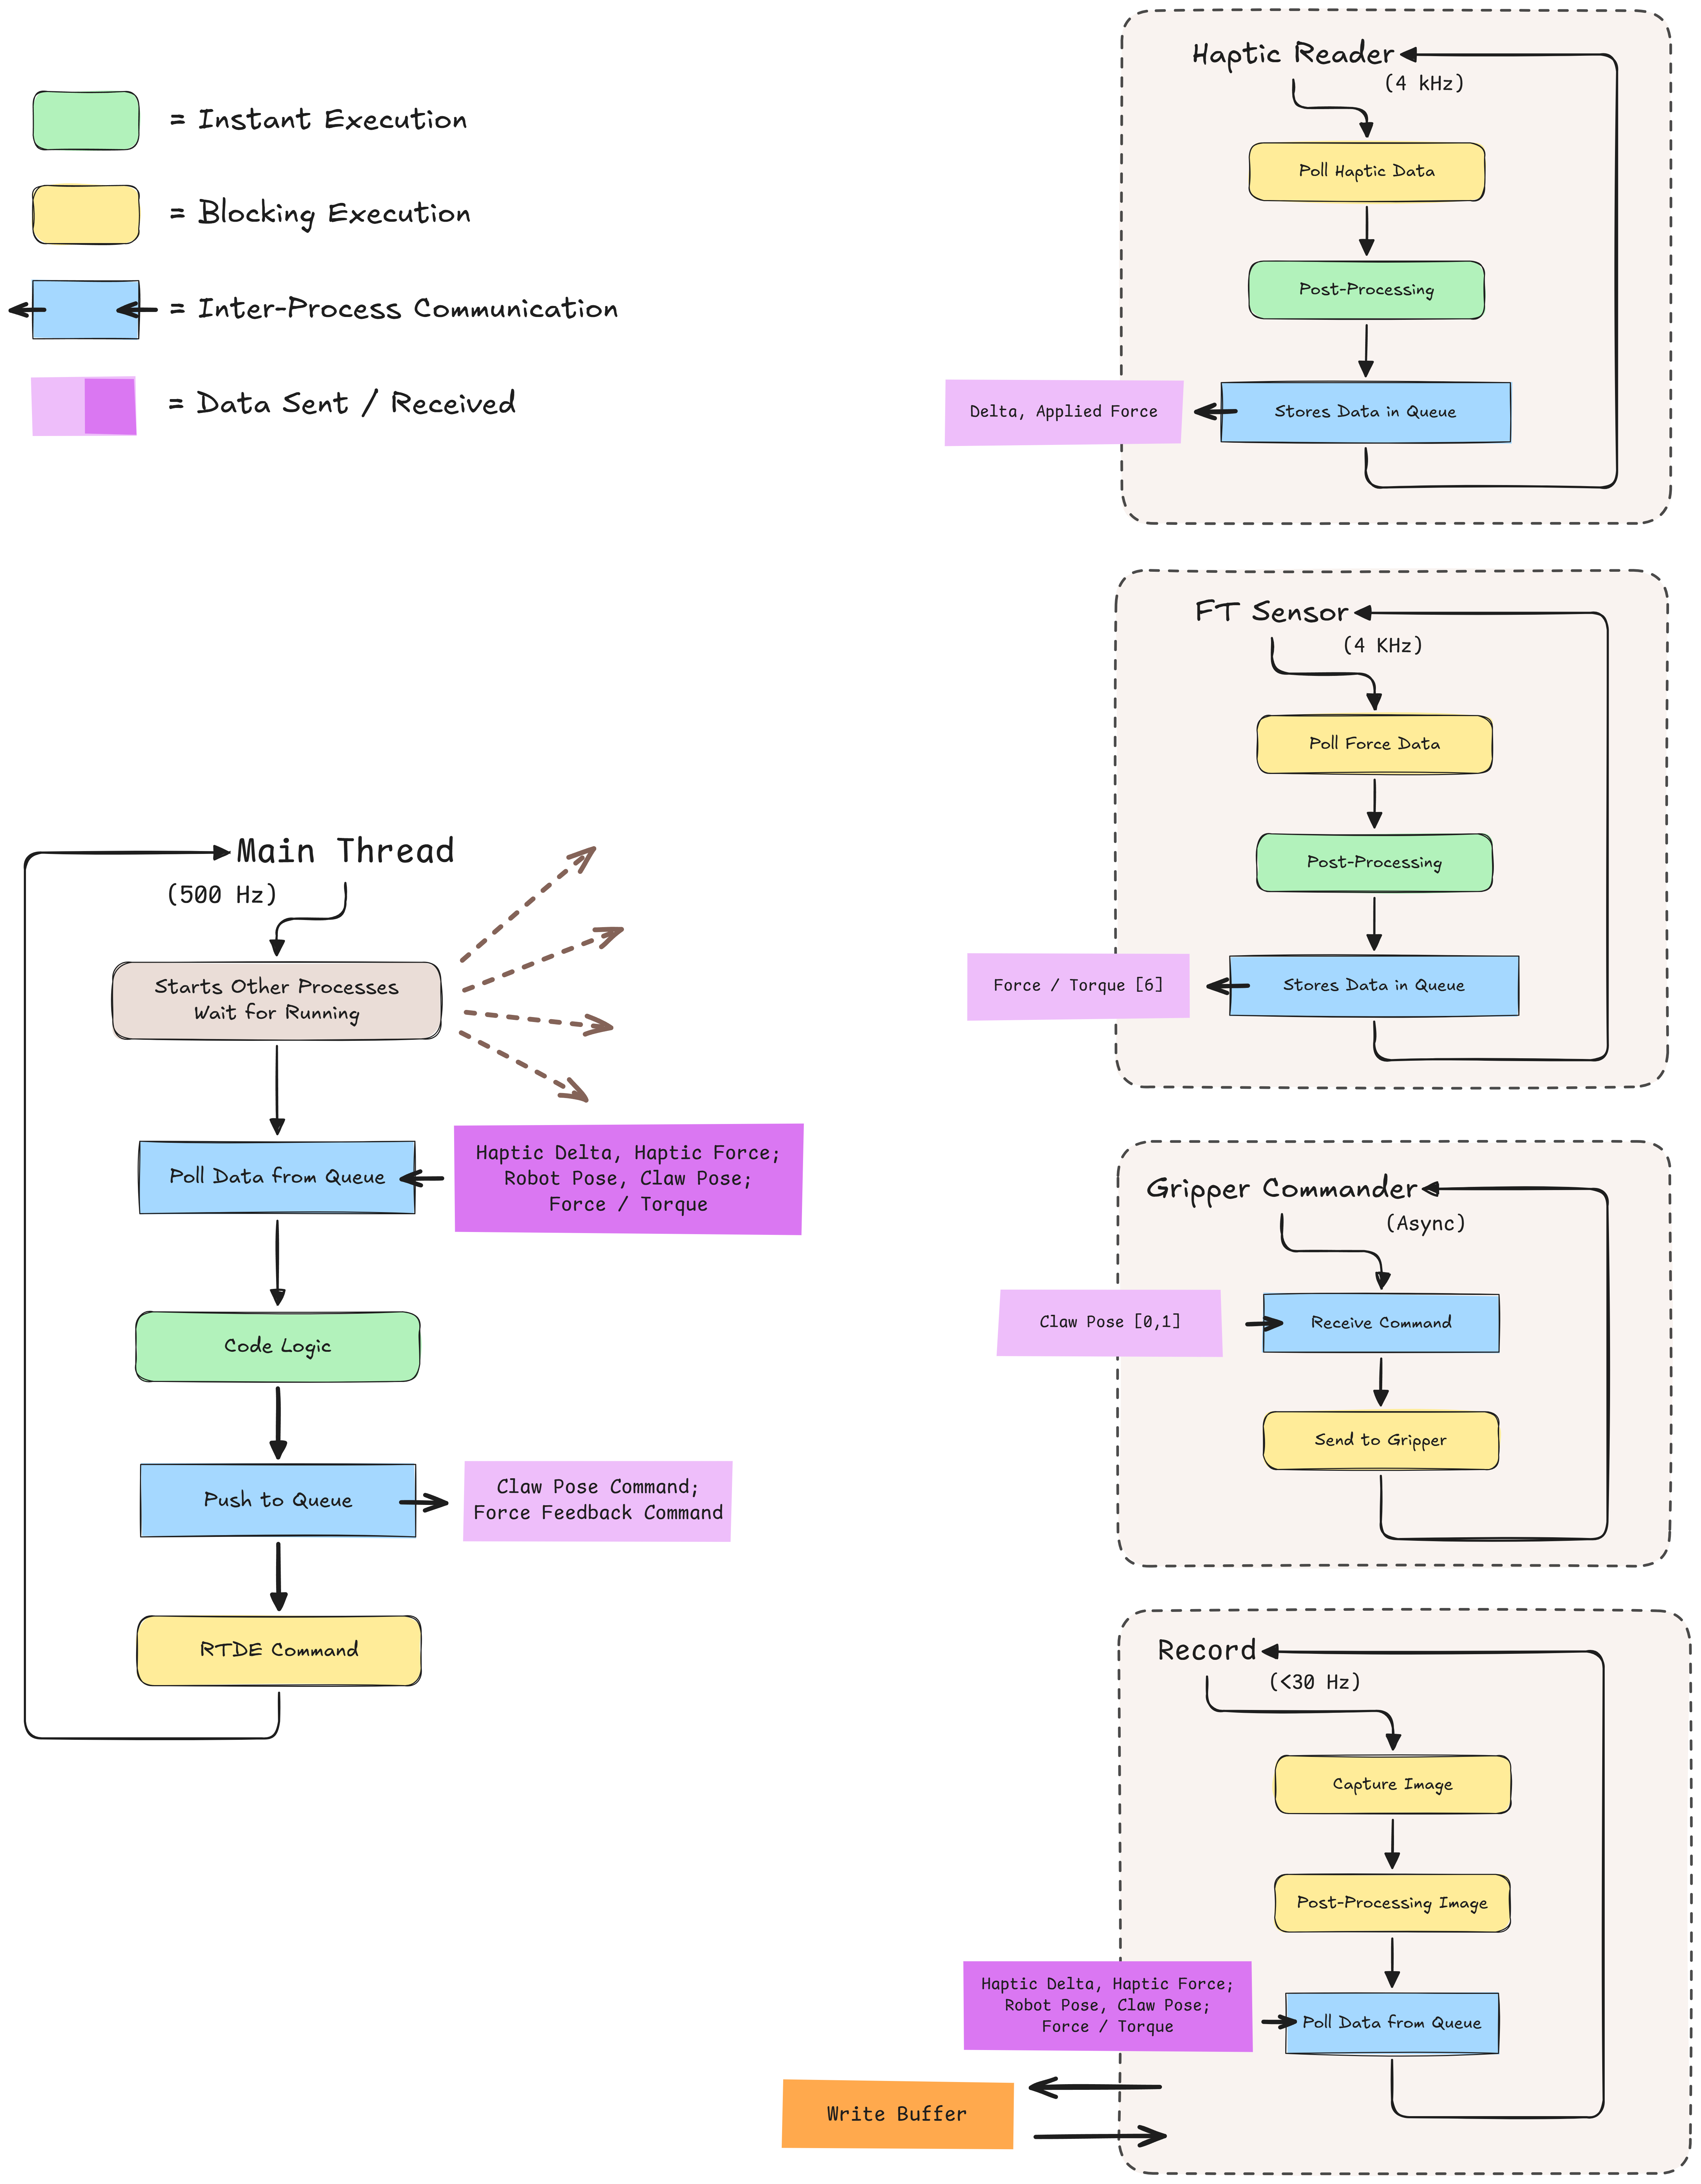
\includegraphics[width=\linewidth]{threading_architecture.png}
\captionof{figure}{Process layout of the refactored runtime.
The main loop exchanges data through queues with the device processes, each running at its device's own rate.}
\label{fig:arch}
\end{minipage}
\footnotetext{\url{\mrurl}}

\section{Force Feedback Proposal}

I am drafting a document, \emph{Force Feedback Refinement}, that aims to improve the current force feedback.
I would like 10 minutes at next Tuesday's meeting to discuss it with the team.

\section{Plan for Next Week}

\begin{enumerate}
    \item \textbf{Teleoperation refactor.} Complete Stages 1 to 3 (Haply teleoperation, gripper and
    force\slash torque sensor). The sensor works but is occasionally unstable, so this proceeds in parallel with
    the MAE inquiry. Test the new code against the old to quantify the improvement. The goal is an observable smoother
    teleoperation demo within the next two weeks.

    \item \textbf{Admittance control.} Integrate Geoffrey's newly implemented admittance-control branch into
    the refactored code. It is reported to partly work, but is very laggy under in the current
    10\,Hz control loop.

    \item \textbf{KIMM collaboration.} Draft the initial research proposal with the group.
\end{enumerate}

\section{Currently Waiting On}

\begin{itemize}
    \item \textbf{Reply from MAE.} Our error report on the force\slash torque sensor has not received reply.
    We now know that the issue is related to static electricity: tightening the sensor's grounding
    wire reduced it, but it still occurs occasionally. We should send MAE a follow-up email with this finding, and to remind them for a reply.

    \item \textbf{Initial project meeting with KIMM.} We will need to ask many questions there to determine the client's needs.
\end{itemize}

\section{Other Projects}

Both projects below are side commitments; my main priority remains the robotics project.

\medskip
\noindent\textbf{Human Motion Planning (led by Dr.~Shu).}
\begin{itemize}
    \item Created the GitLab repository for the project.
    \item Converted his research proposal into a \LaTeX{} document.
    \item Uploaded his draft code and created a conda Python environment for future development.
    The environment runs on laptops, the lab workstation and the NRC Trixie HPC cluster.
    \item I am waiting for his thoughts on the next steps, and expect to meet with him next week.
\end{itemize}

\noindent\textbf{DRDC Human-Swarm Teaming (Shunyu).}
From what I understand, the client complains that OpenAI's Whisper model (tiny, without
fine-tuning or prompting) performs poorly in their use case: it mis-transcribes domain vocabulary such as
callsigns, coordinates and units, and cannot understand the commander's intent reliably.
I have offered to help and agree that fine-tuning is the most promising approach.
I will work with Shunyu to draft a proposed fine-tuning workflow together, starting from measuring the performance of non-training baseline approaches. We hope to discuss it next week.

\end{document}
